\chapter{Experiments}
\label{ch:experiments}

\section{Datasets}
\label{sec:ds}

In this section we consider datasets that are separated in two opposing communities. The information about the opinions of each member of this community is known. Thus, we can assign internal opinions -1 and 1 to the nodes depending on their community membership\cite{tsapMatakosTerzi}.  We consider the following.

\begin{enumerate}

  \item The Karate dataset, that represents the friendships between the members of a karate club at a US university. This network is split in two equal size polarized communities around two rival karate instructors.
  
  \item The Books dataset, that is a network of US politics books. These books were published near the 2004 presidential election and sold by Amazon. These Books are classified as "Liberal", "Conservative", or "Neutral".  There are in total 43 liberal books, 49 conservative and 13 neutral.
  
  \item The Blogs dataset, a network of hyperlinks between online blogs on US politics. Blogs are classified as either Liberal or Conservative.
  
  \item The Elections dataset, this dataset is the network between the Twitter followers of Hillary Clinton and Donald Trump collected in the period 15/12/2016-15/01/2017 – around the time of the 2016 presidential elections. Members of this network are assigned an internal opinion of 1 or -1 based on which one of the two candidates they follow. We took a subsampled portion that has be created by Matakos, et al \cite{tsapMatakosTerzi}.
    
  \item The beefban dataset, a  hashtag that Twitter users used in March 2015 to signal that their posts referred to a decision by the Indian government about the consumption of beef meat in India.
  
  \item The GermanWings dataset, a  hashtag that Twitter users used after the crash of GermanWings Flight 9525.
  
\end{enumerate}


\section{Dataset statistics}
\label{sec:stats}

\begin{table}[H]
 \centering
 \caption{Statistics}
 \label{tab:statistics}
 \begin{tabular}{| l || l | l | l | l |}
 \hline
  Name & \# of Nodes & \# of Edges & Avg. Degree & $\pi(z)$\\
  \hline
  \hline
  Karate & $34$ & $78$ & 4.5882 &  0.33964\\
  \hline
    books & $105$ & $441$ & 8.4 &  0.43429\\
  \hline
    beefban & $799$ & $6026$ & 15.0839 &  0.30326\\
  \hline
  polblogs & $1490$ & $16718$ & 22.4403 &  0.30983\\
  \hline
  GermanWings & $2111$ & $7329$ & 6.9436 &  0.44479\\
  \hline
  ClintonTrump & $2832$ & $18551$ & 13.1010 &  0.07582\\
  \hline
 \end{tabular}
 \end{table}
 
\vspace{20pt}
\clearpage

\section{Experiments}
\label{sec:experim}

All experiments were made with an 2,7 GHz Dual-Core Intel Core i5 on the PyCharm IDE. We can only experiment with the $Karate$ and the $Books$ dataset on all the heuristics. The $Greedy$ algorithm cannot run on the rest of the datasets because they contain thousands of nodes. The $Greedy$ algorithm needs to consider changes in the network structure so it is impossible to compute the polarization so many times.
\\
\\ 
The $FirstTopGreedy$ and the $Expressed Opinion$ can run in all datasets and us with a fairly good decrease in polarization compared to the batch algorithms. This decrease can be greater if we consider edge additions that are proportional to the size of the dataset. Greater number of edges would make $FirstTopGreedy$ nonrunnable. The $Expressed Opinion$ can run in our larger datasets with big number of additions.
\\
\\
In addition to the heuristics we use two random algorithms. The $Random$, that chooses random edges from all possible combinations and the $RandomDifferent$. The second one chooses random edges between different $z$ opinions. More specifically edges that the multiplication of their expressed opinions is negative ($z_u*z_v < 0$). 
\\
\\
\noindent We start by applying the heuristics described at~\ref{ch:algorithms} in our 6 datasets. The algorithms perform as expected. The greedy ones have better results but are expensive in time. We can not run the $Greedy$ algorithms in larger datasets due to time limitations. In figure~\ref{fig:heuristics_small} we can see the charts that compare the decrease of the polarization index of the heuristics.
\clearpage

\begin{figure}[!htbp]
	\begin{center}
	\advance\leftskip-1.3cm
	\captionsetup{justification=centering,margin=2cm}
	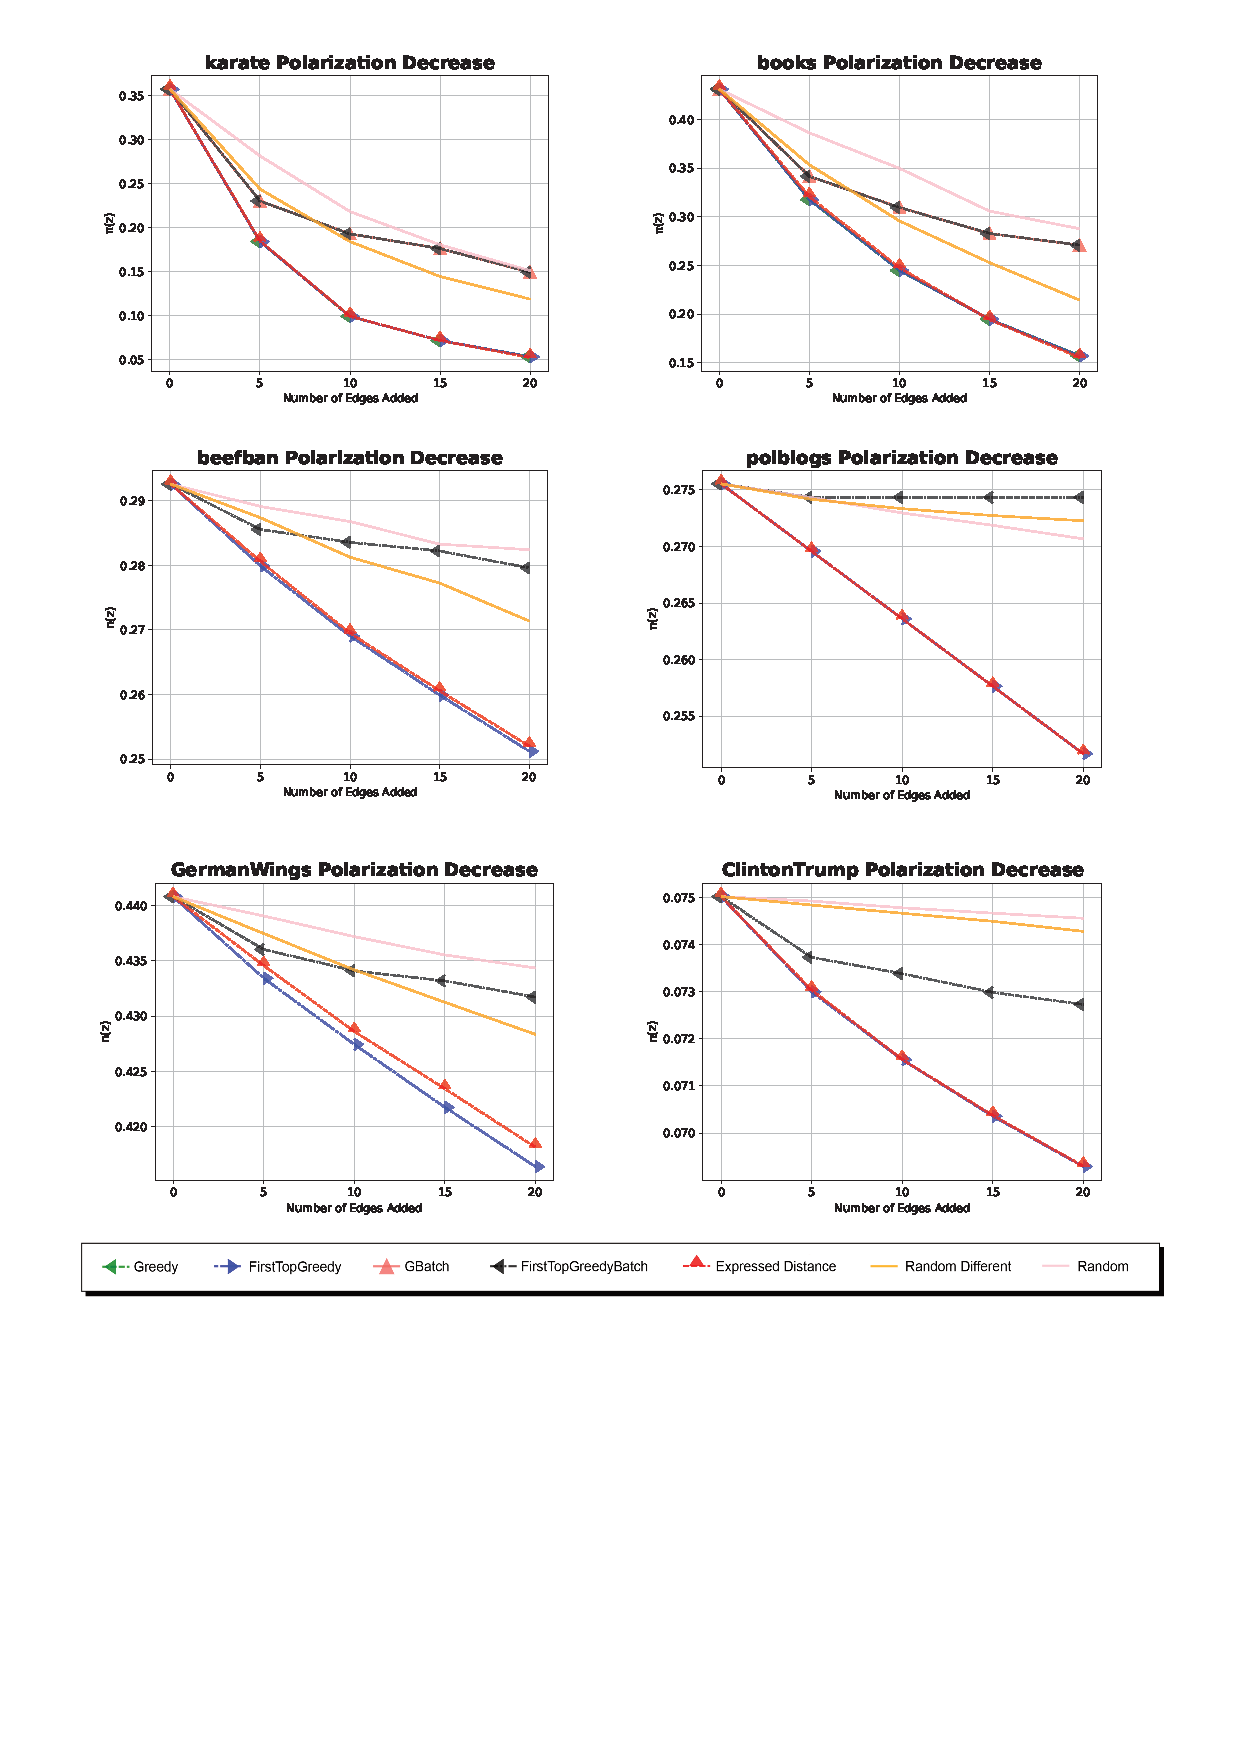
\includegraphics[width=1.2\textwidth]{Figures/heuristics}
	\caption{Comparison of the heuristics between datasets}
	\label{fig:heuristics_small}
	\end{center}
\end{figure}
\clearpage

\begin{itemize}
  \item The Expressed Opinion heuristic, that is based on the distance of the opinions, performs very well, similar to $Greedy$ and is cheap on time.
  \item Batch algorithms perform very poorly, even worse than Random. When adding a new edge the Batch algorithms do not recompute the $z$ vector. That means that the heuristic has a false view of the opinions of the network. For example in a batch version of the $ExpressedOpinion$ the nodes that have the most extreme opinions of each side are reused even if their value is changed after an addition and are no longer the ones with the most extreme values.
 \end{itemize}
 
 \section{A Visualisation of Edge Additions}
\label{sec:vis}
In the figures bellow we can see the karate graph before and after adding the top 10 edges proposed by the $Greedy$ algorithm. Blue nodes represent expressed opinions $\epsilon [-1,0)$, red nodes represent expressed opinions $\epsilon (0,1]$ and size shows how central a node is. The size has been computed with the help of the pagerank algorithm. The green edges are the additions proposed by the algorithm. We can clearly see that before adding edges of different opinions the network is polarized in two communities.
\\
\\
\begin{figure}[!htbp]
	\centering
	\begin{subfigure}[t]{0.45\textwidth}
		\centering
		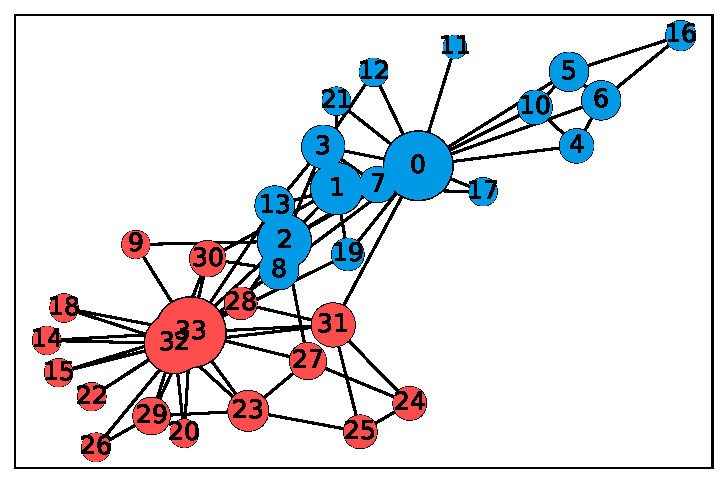
\includegraphics[height=0.2\textheight]{Figures/before_pol}
		\caption{The karate graph}
		\label{subfig:before_pol}
	\end{subfigure}
	\hfill
	\begin{subfigure}[t]{0.45\textwidth}
		\centering
		\captionsetup{justification=centering}
		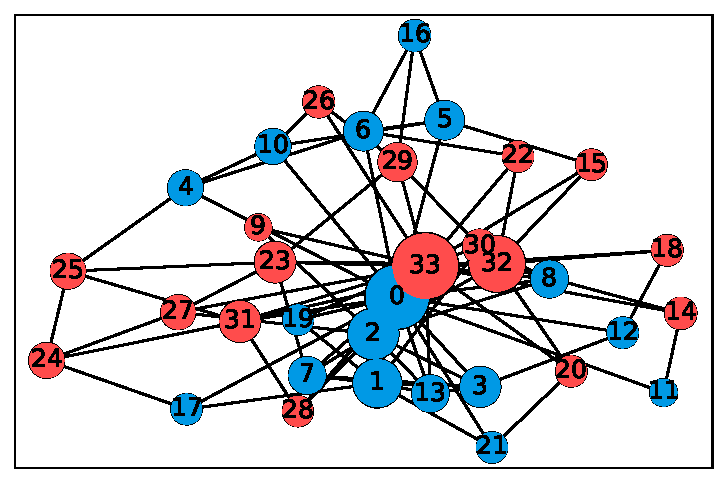
\includegraphics[height=0.2\textheight]{Figures/after_pol}
		\caption{The karate graph after adding 10 edges proposed by $Greedy$}
		\label{subfig:after_pol}
	\end{subfigure}
	\vspace{20pt}
	\hfill
	\caption{Edge addition between opposed opinions.}
	\label{fig:top-10-karate}
\end{figure}
\\
\clearpage

\noindent We can continue by visualising and comparing edges additions between the rest of the algorithms. We observe in the comparison of the choices of $Greedy$ and $GreedyBatch$ that the second reuses the same nodes. This is aligned with the way batch algorithms work. By not recomputing the $z$ vector they will always choose the same nodes thinking they are the best candidates. We proceed to compare the $ExpressedOpinion$ at with $FirstTopGreedy$ and $Greedy$. We can clearly see that the nodes that are being selected are discrete and they are not reused. 
\\
\\
To conclude with these visualisations, when we compare heuristics that do not recompute the $z$ vector we will observe that some nodes participate in edges that will be added multiple times. If the heuristics recompute the $z$ vector the nodes will not be reused.
\\
\\

\begin{figure}[!htbp]
	\centering
	\begin{subfigure}[t]{0.49\textwidth}
		\centering
		 \advance\leftskip-0.9cm
		 \captionsetup{justification=centering}
		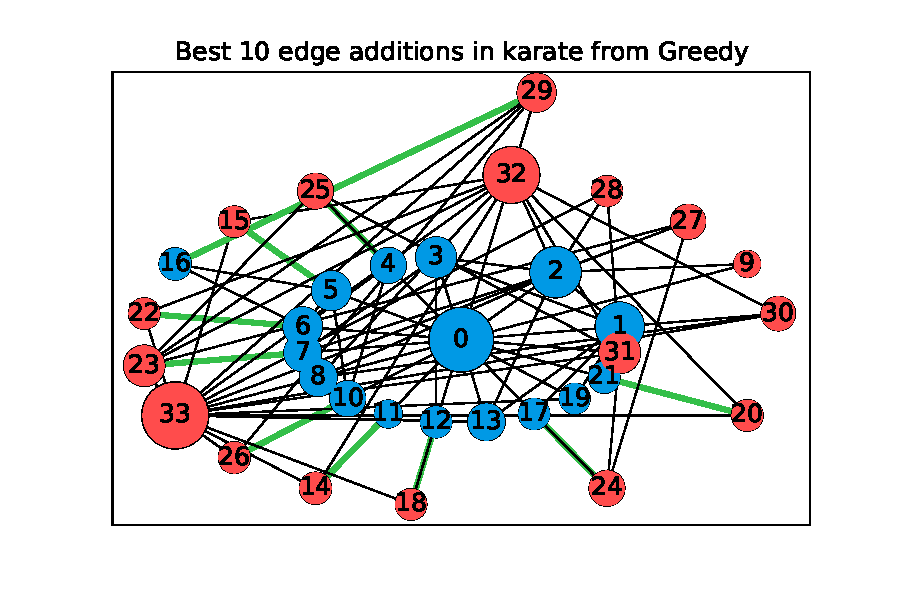
\includegraphics[height=0.25\textheight]{Figures/karate_Greedy_edge_vis}
		\caption{The karate graph after adding 10 edges proposed by $Greedy$}
		\label{subfig:greedy}
	\end{subfigure}
	\hfill
	\begin{subfigure}[t]{0.49\textwidth}
		\centering
		\captionsetup{justification=centering}
		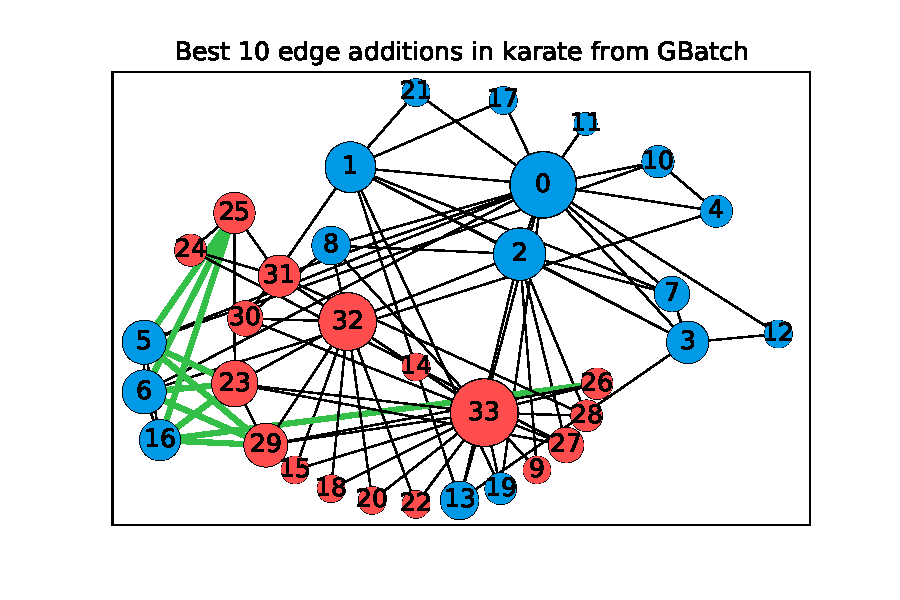
\includegraphics[height=0.25\textheight]{Figures/karate_GBatch_edge_vis}
		\caption{The karate graph after adding 10 edges proposed by $GreedyBatch$}
		\label{subfig:gbatch}
	\end{subfigure}
	\vspace{20pt}
	\hfill
	\caption{Difference of edges between $Greedy$ and $GreedyBatch$}
	\label{fig:top-10-karate}
\end{figure}

\clearpage

\begin{figure}[!htbp]
	\centering
	\begin{subfigure}[t]{0.49\textwidth}
		\centering
		 \advance\leftskip-0.9cm
		 \captionsetup{justification=centering}
		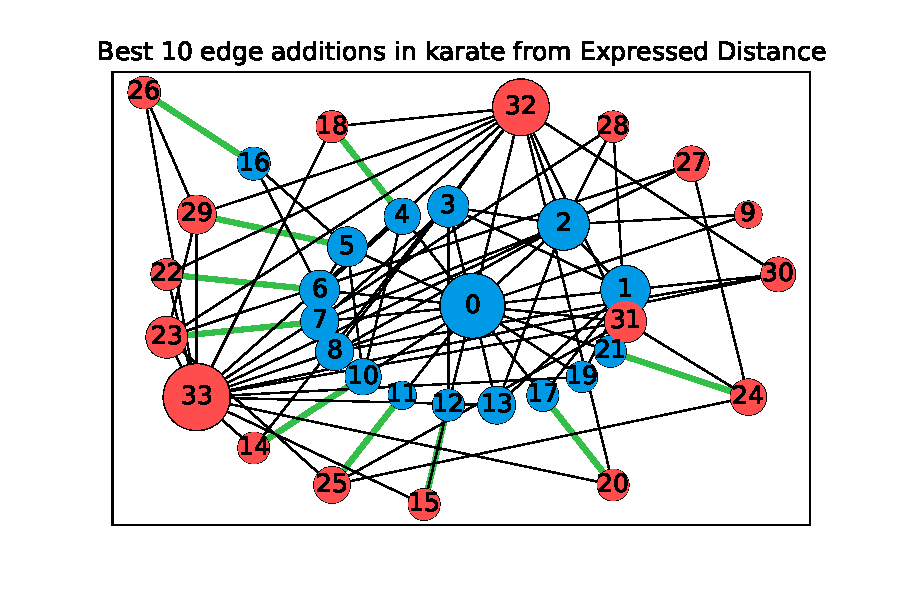
\includegraphics[height=0.25\textheight]{Figures/karate_Expressed Distance_edge_vis}
		\caption{The karate graph after adding 10 edges proposed by $ExpressedOpinion$}
		\label{subfig:g2}
	\end{subfigure}
	\hfill
	\begin{subfigure}[t]{0.49\textwidth}
		\centering
		\captionsetup{justification=centering}
		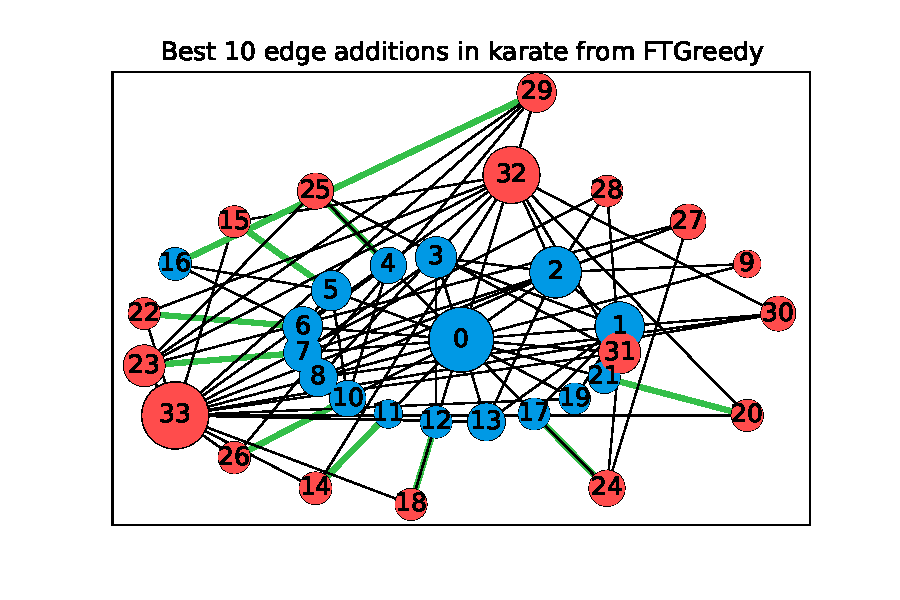
\includegraphics[height=0.25\textheight]{Figures/karate_FTGreedy_edge_vis}
		\caption{The karate graph after adding 10 edges proposed by $FirstTopGreedy$}
		\label{subfig:ftg}
	\end{subfigure}
	\vspace{20pt}
	\hfill
	\caption{Difference of edges between $ExpressedOpinion$ and $FirstTopGreedy$}
	\label{fig:top-10-karate3}
\end{figure}

\vspace{30pt}

\begin{figure}[!htbp]
	\centering
	\begin{subfigure}[t]{0.49\textwidth}
		\centering
		 \advance\leftskip-0.9cm
		 \captionsetup{justification=centering}
		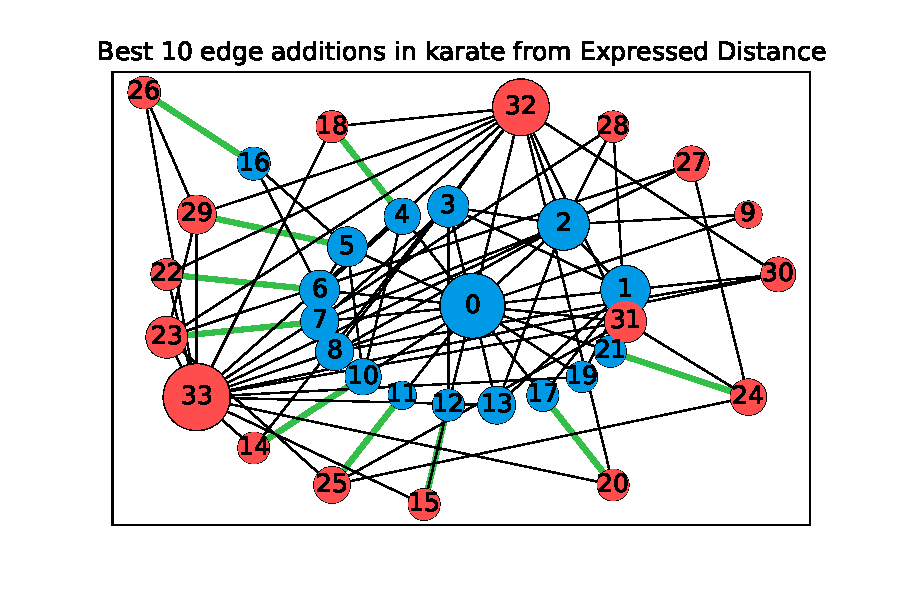
\includegraphics[height=0.25\textheight]{Figures/karate_Expressed Distance_edge_vis}
		\caption{The karate graph after adding 10 edges proposed by $ExpressedOpinion$}
		\label{subfig:ge3}
	\end{subfigure}
	\hfill
	\begin{subfigure}[t]{0.49\textwidth}
		\centering
		\captionsetup{justification=centering}
		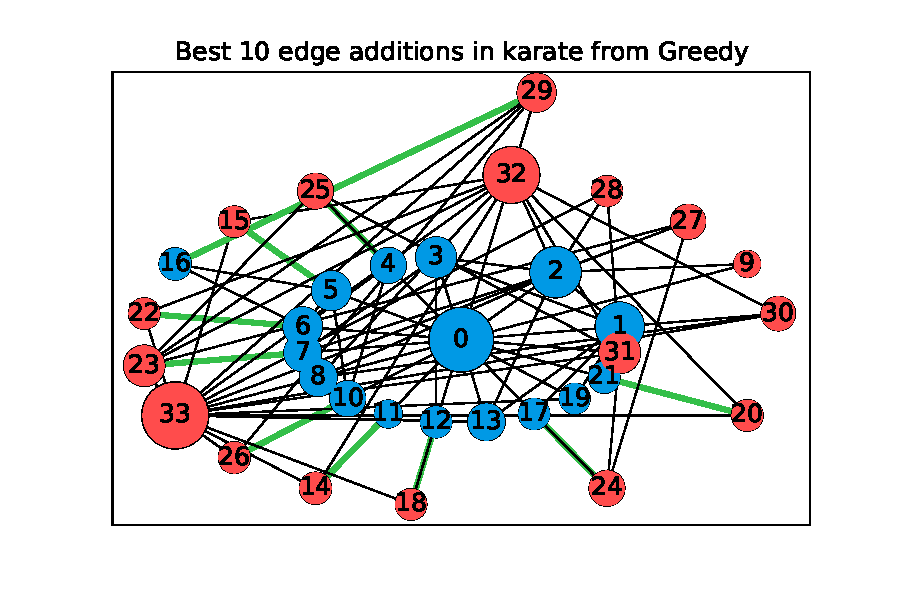
\includegraphics[height=0.25\textheight]{Figures/karate_Greedy_edge_vis}
		\caption{The karate graph after adding 10 edges proposed by $Greedy$}
		\label{subfig:g3}
	\end{subfigure}
	\vspace{20pt}
	\hfill
	\caption{Difference of edges between $ExpressedOpinion$ and $Greedy$}
	\label{fig:top-10-karate3}
\end{figure}

\clearpage


\section{Measuring the median probability}		
\label{sec:median}

We measure the median probability of the edges selected by the heuristics and compare it to the ones that were edited to include acceptance probabilities. We expect that the edited heuristics will have a higher median value. A new algorithm called $maxProb$ is included that chooses an edge if it is among the edges with the highest acceptance probabilities. This sets an upper limit for the mean probability by having the highest mean probability among all heuristics. This will help us compare the edited heuristics that use acceptance probabilities. We want them to have a relatively higher acceptance probability among the edges they choose. There is a clear increase in the mean probability of the edges the edited heuristics choose.

\begin{figure}[!htbp]
	\begin{center}
	\advance\leftskip-1.5cm
	\captionsetup{justification=centering,margin=2cm}
	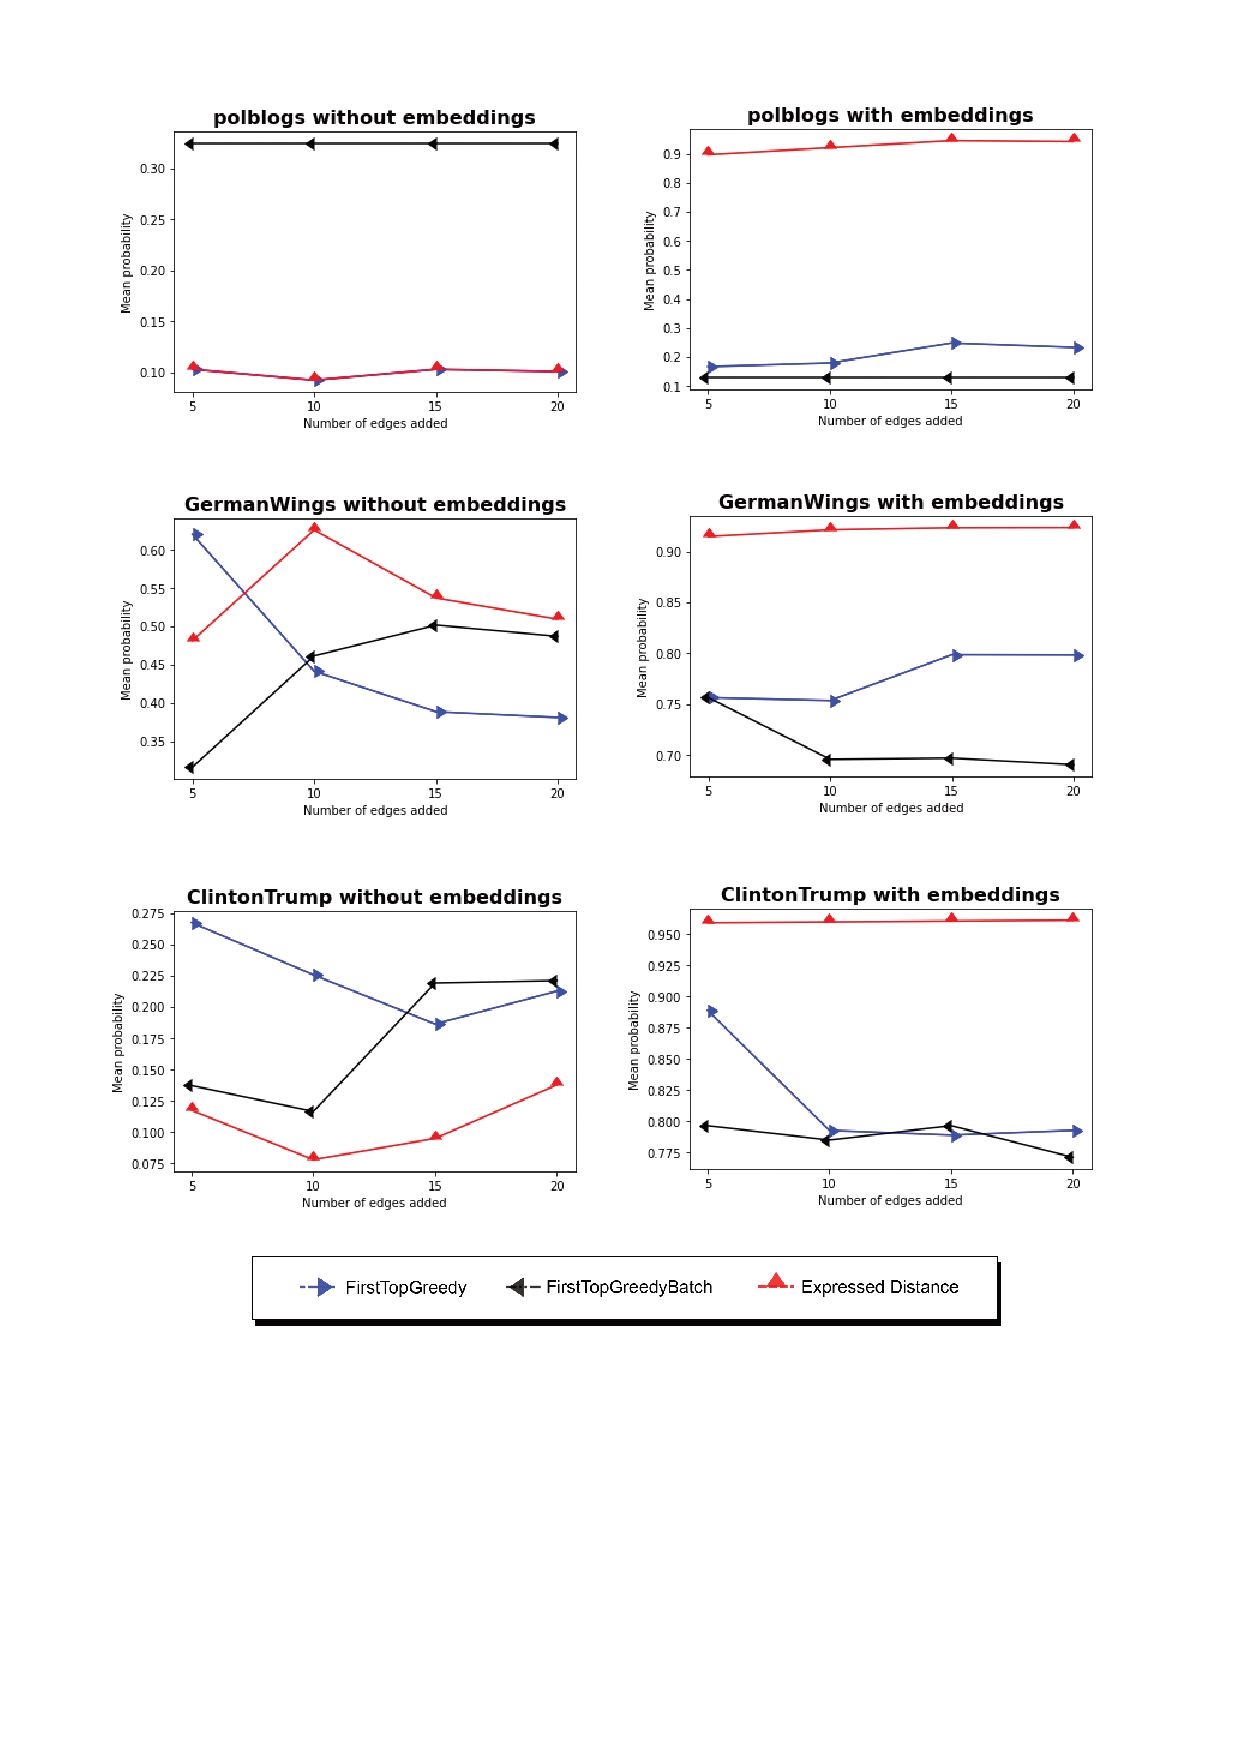
\includegraphics[width=1.2\textwidth]{Figures/m2}
	\caption{Comparison of the median probability}
	\label{m1}
	\end{center}
\end{figure}

\clearpage

\begin{figure}[!htbp]
	\begin{center}
	\advance\leftskip-1.3cm
	\captionsetup{justification=centering,margin=2cm}
	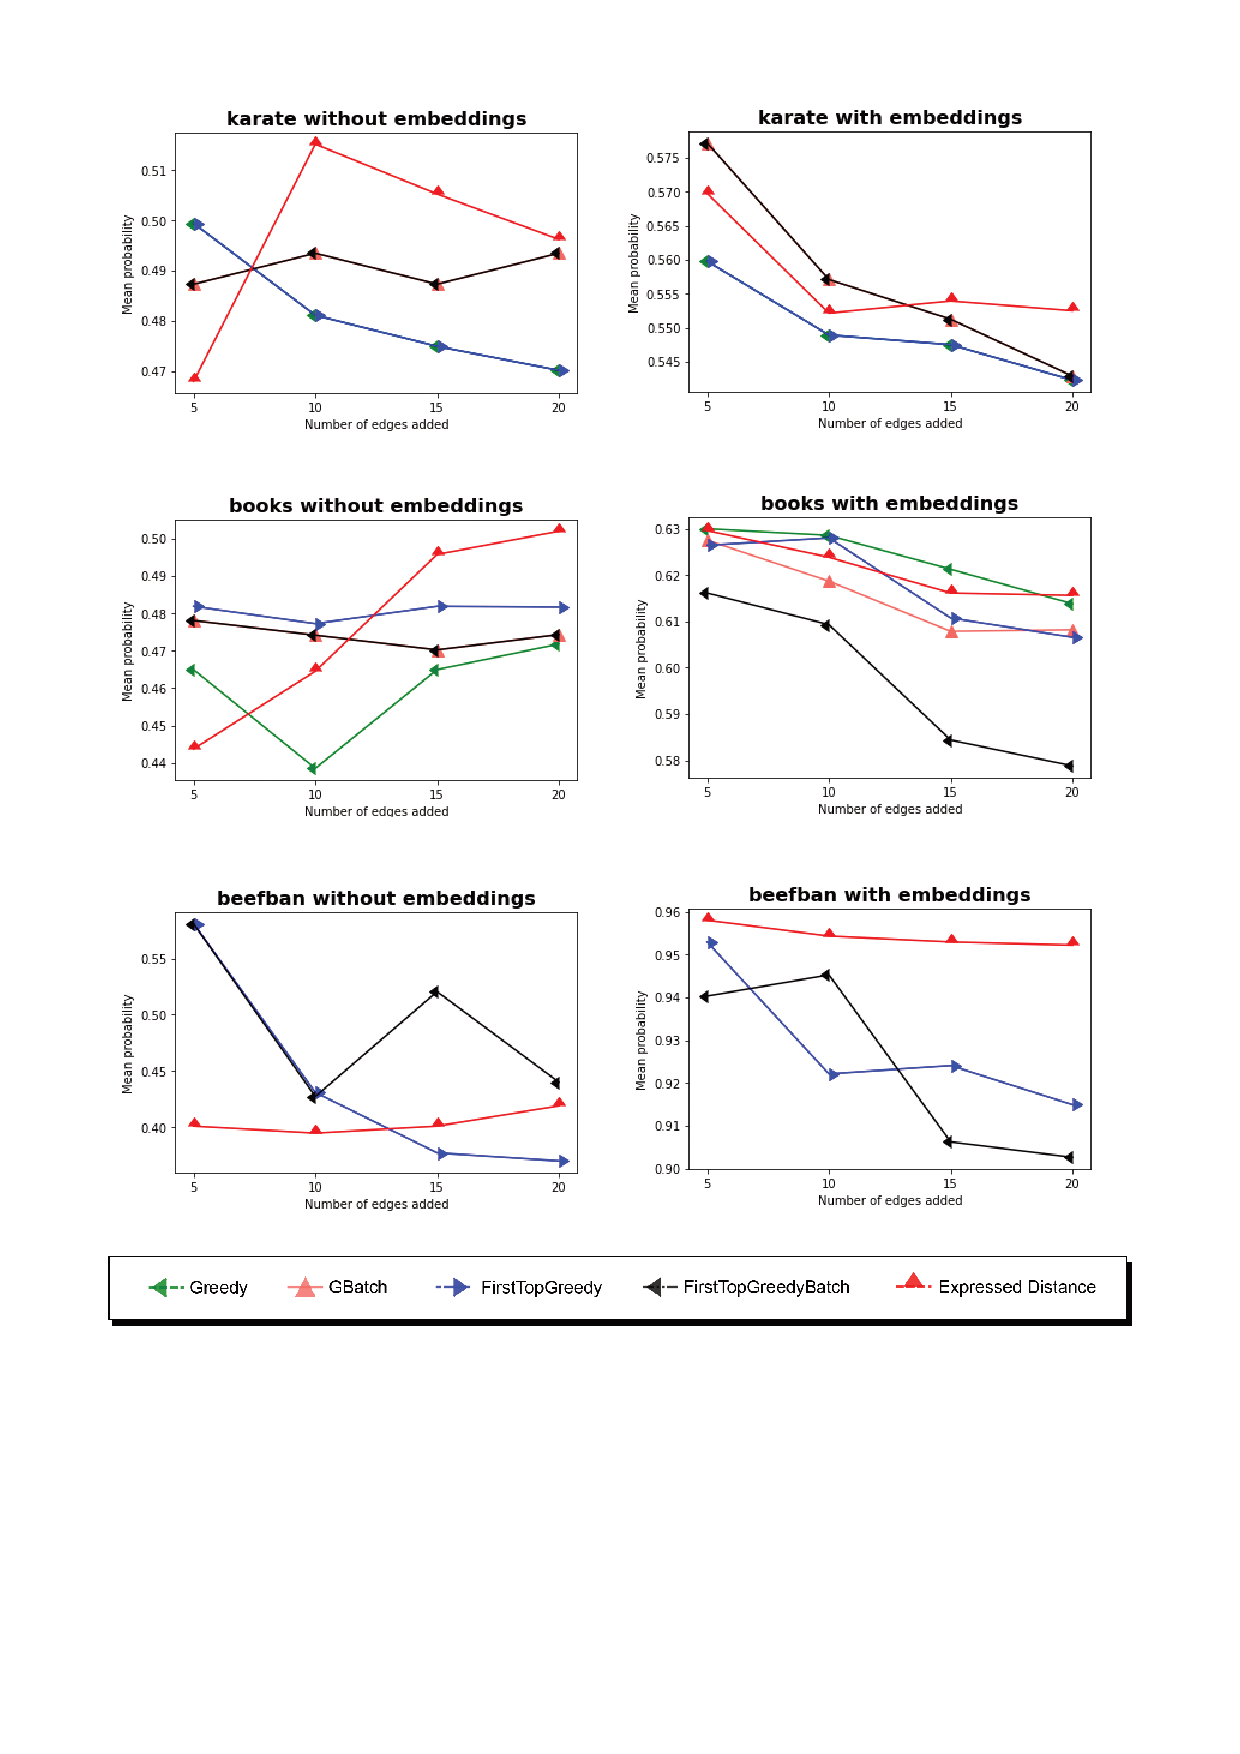
\includegraphics[width=1\textwidth]{Figures/m1}
	\caption{Comparison of the median probability}
	\label{m2}
	\end{center}
\end{figure}
\clearpage

\section{Comparing all the heuristics}		
\label{sec:all}

In this section we compare all the algorithms together, $maxProb$ is also displayed in the chart. As mentioned before we want the edited heuristics to have a higher acceptance probability among the edges they choose and this can be seen in the figures~\ref{m2} and~\ref{m1}. In these graphs we can see that the polarization is not reduced as much as the original heuristics. This is the tradeoff that the acceptance probabilities create. If we try to reduce the polarization index in a network by not including acceptance probabilities there would be a chance that the decrease would not be as good because individuals could reject these recommendations.
 
\begin{figure}[!htbp]
	\begin{center}
	\advance\leftskip-1.5cm
	\captionsetup{justification=centering,margin=2cm}
	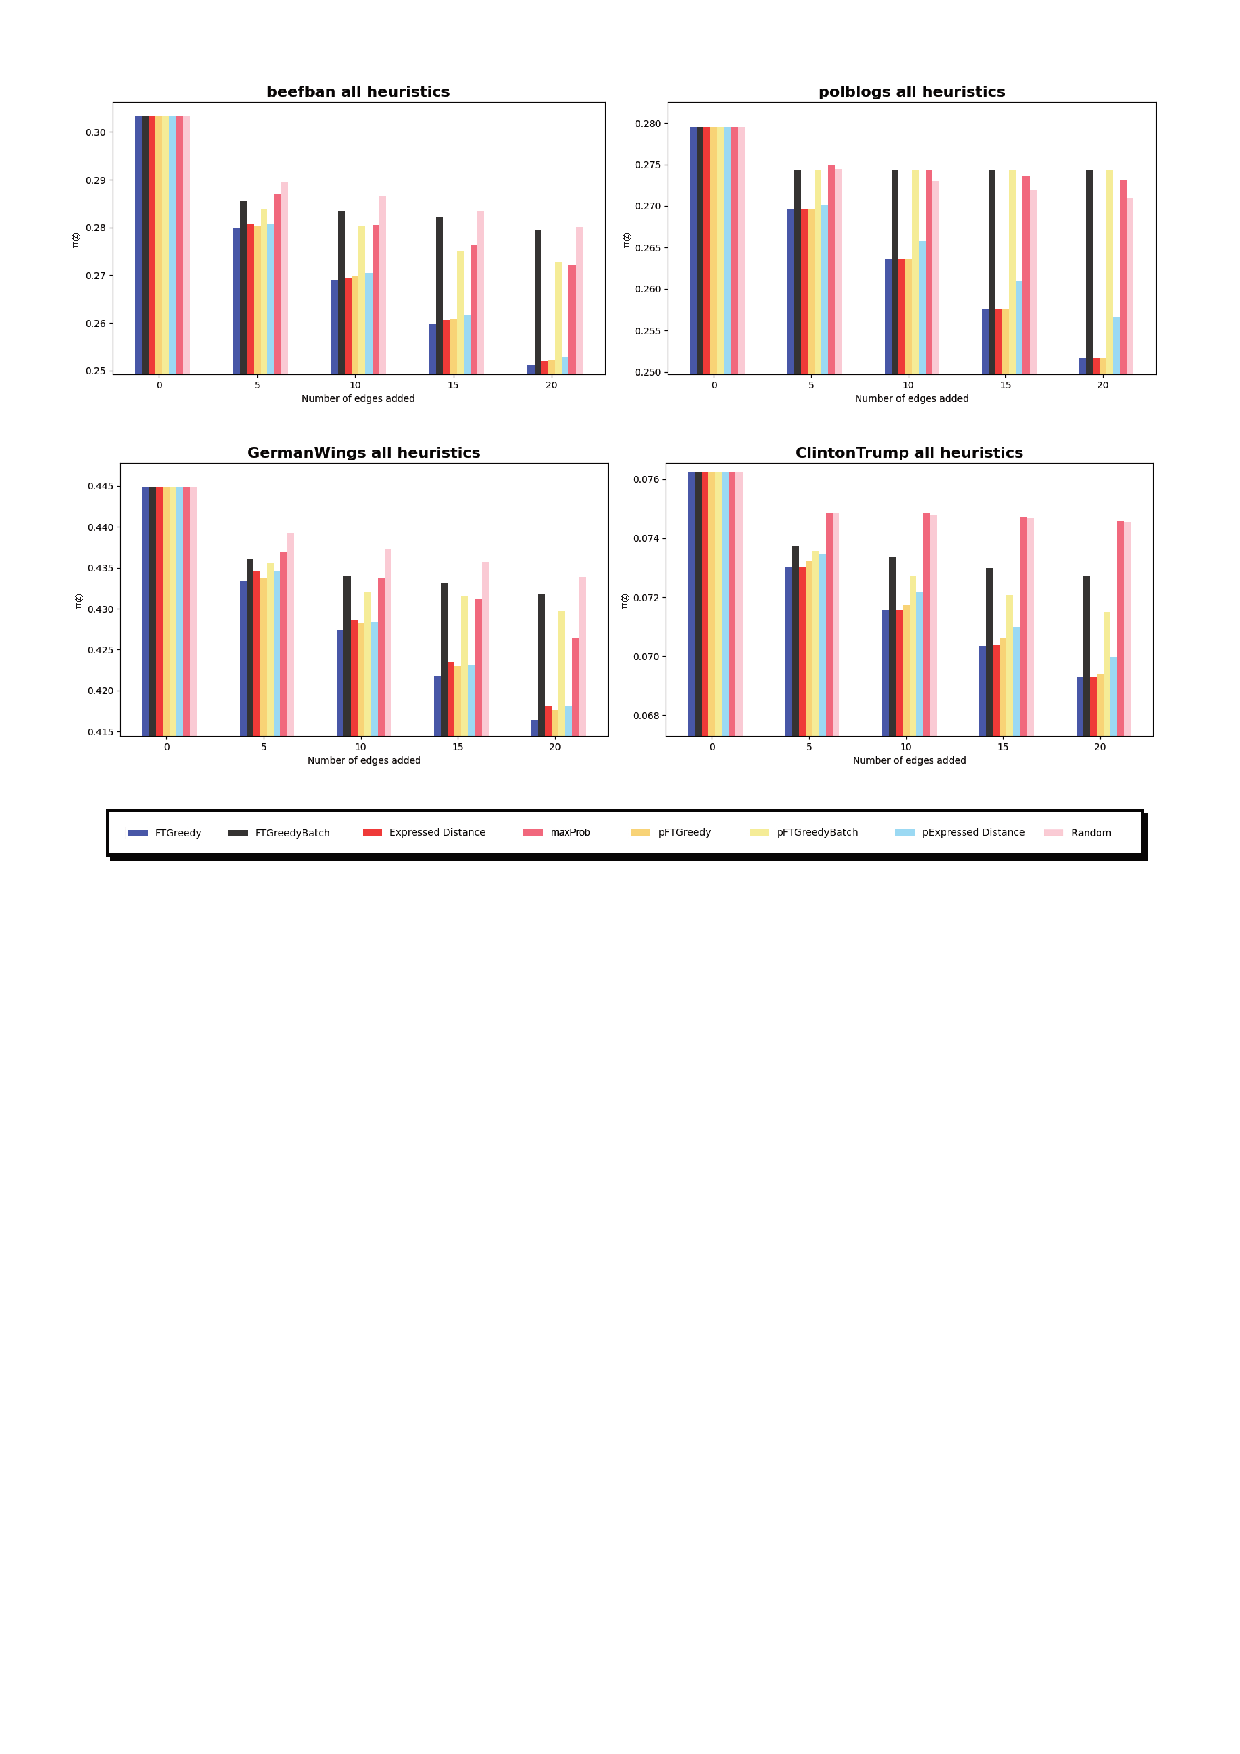
\includegraphics[width=1.2\textwidth]{Figures/all2}
	\caption{Comparison of all the heuristics}
	\end{center}
	\label{all1}
\end{figure}

\clearpage

\begin{figure}[!htbp]
	\begin{center}
	\advance\leftskip-1.3cm
	\captionsetup{justification=centering,margin=2cm}
	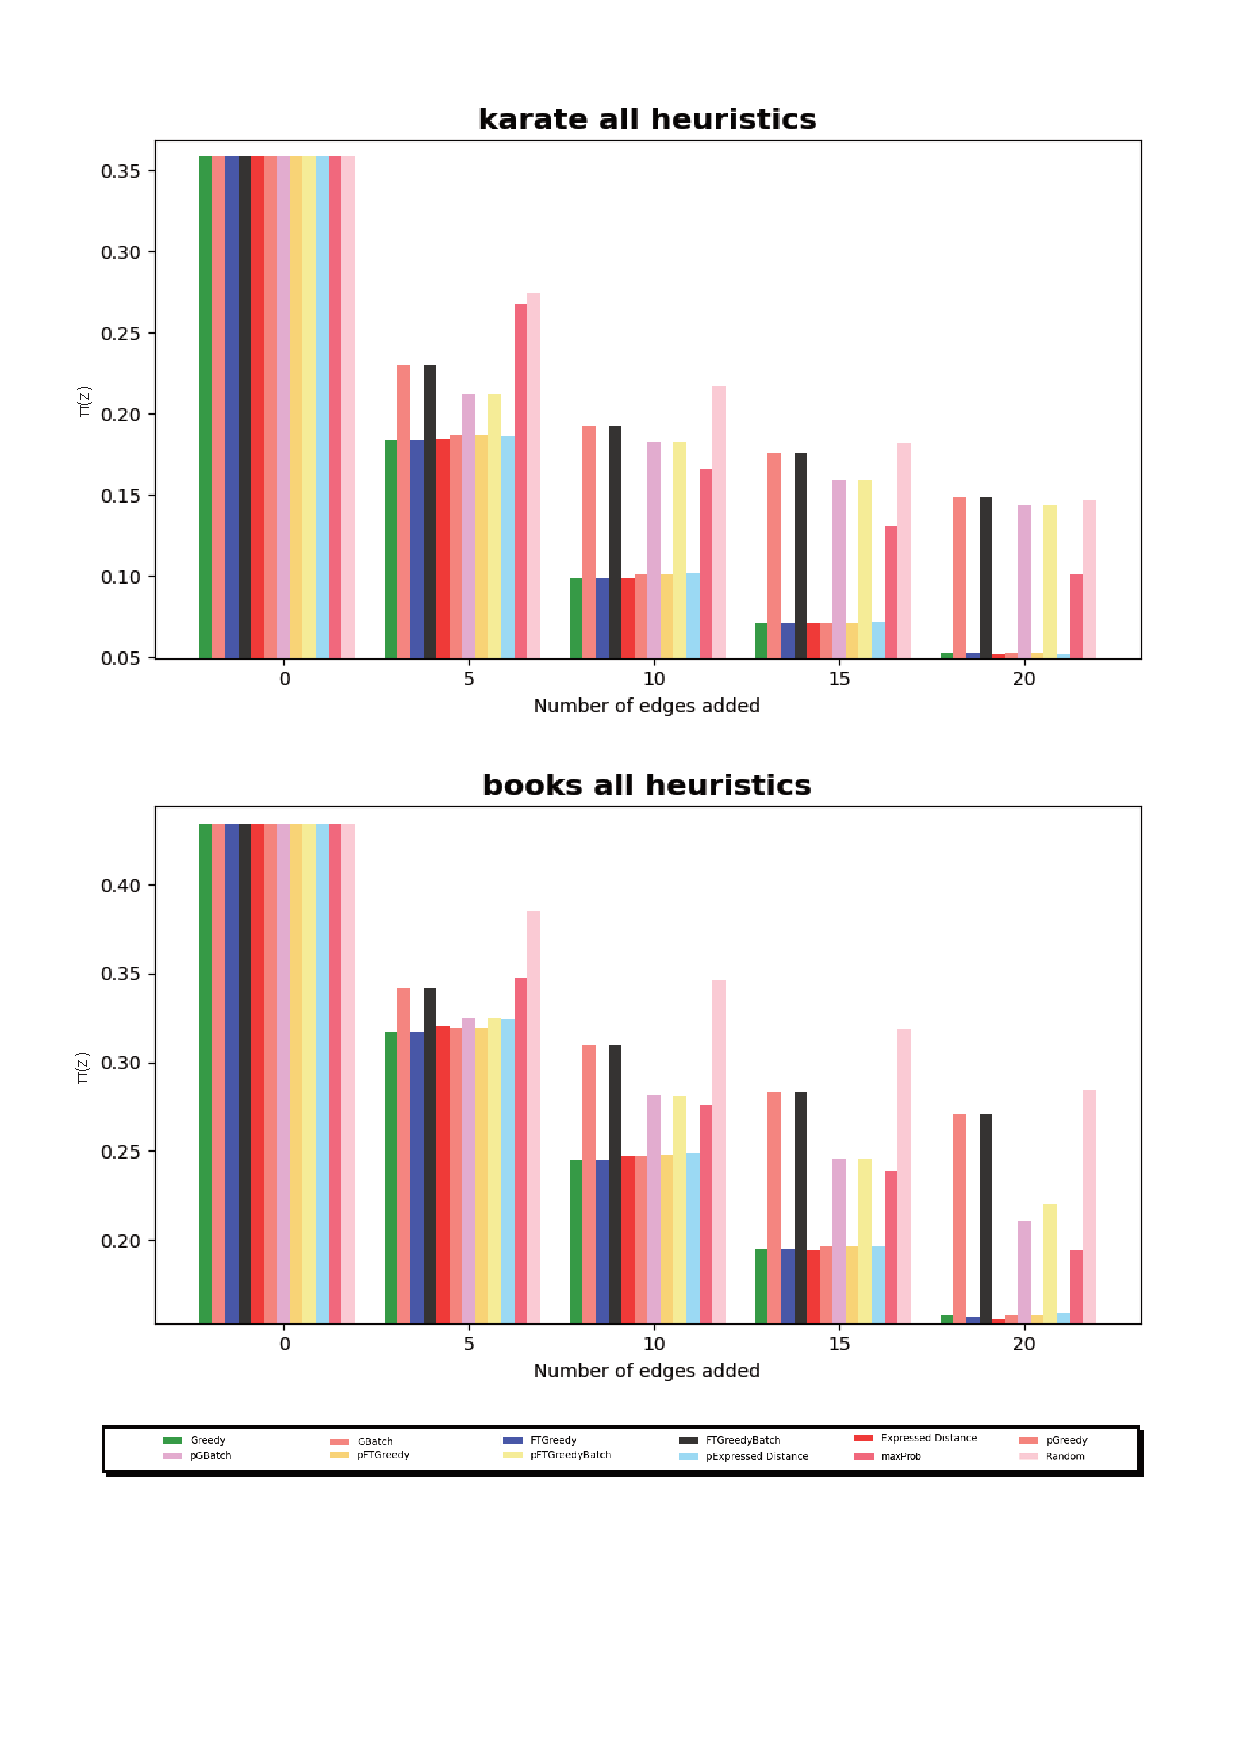
\includegraphics[width=1\textwidth]{Figures/all1}
	\caption{Comparison of all the heuristics}
	\end{center}
	\label{all2}
\end{figure}

